\begin{figure}[tbp]
\centering
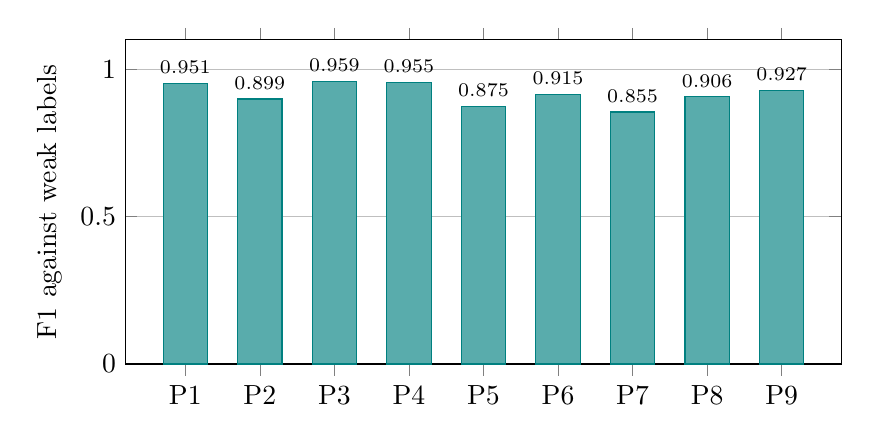
\begin{tikzpicture}
\begin{axis}[width=0.88\linewidth,height=5.7cm,ybar,bar width=16pt,ymin=0,ymax=1.10,
  ylabel={F1 against weak labels},symbolic x coords={P1,P2,P3,P4,P5,P6,P7,P8,P9},xtick=data,
  ymajorgrids=true,nodes near coords,nodes near coords style={font=\scriptsize,/pgf/number format/fixed,/pgf/number format/precision=3}]
\addplot[fill=teal!65,draw=teal] coordinates {(P1,0.9511)(P2,0.8992)(P3,0.9588)(P4,0.9549)(P5,0.8751)(P6,0.9145)(P7,0.8551)(P8,0.9064)(P9,0.9272)};
\end{axis}
\end{tikzpicture}
\caption{F1 by principle for the recovered classifier. A higher bar means a better balance of precision and recall against the recorded weak labels. P7 has 69 test examples, compared with 1,715 for P3. Table~\ref{tab:per_principle} gives all example counts and measures.}
\label{fig:per_principle}
\end{figure}
